% Regular polygons
\documentclass[tikz,border=10pt]{standalone}
\usepackage{tikz}
\usetikzlibrary{shapes,calc,arrows,through,intersections}
\usetikzlibrary{decorations.pathmorphing}
\usetikzlibrary{decorations.markings}
\usepackage{calc}

\begin{document}

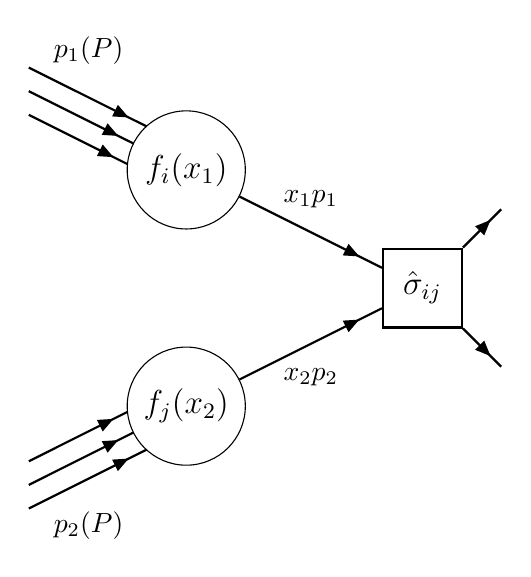
\begin{tikzpicture}
  % \draw[step=1.0,thin,gray!40] (0,0) grid (10,10);

  \node[circle, draw, minimum size=1.5cm] (circleANode) at  (4,7) {\large $f_i(x_1)$};
  \node[circle, draw, minimum size=1.5cm] (circleBNode) at  (4,4) {\large $f_j(x_2)$};
  \path[name path=circleA, thick] (4,7) circle [radius=0.75];
  \path[name path=circleB, thick] (4,4) circle [radius=0.75];

  \draw[thick] (7,5.5) node[draw,rectangle,minimum width=1.0cm,minimum height=1.0cm] (C) {\large $\hat \sigma_{ij}$};

  \path[name path=A1] (2,8.3) -- (4,7.3);
  \draw [postaction={decorate, decoration={markings, mark=at position 0.8 with {\arrow[scale=0.7,xshift=3.333pt]{triangle 45}}}},name intersections={of=A1 and circleA}, thick]  (2,8.3) -- (intersection-1) node[above right,very near start] {$p_1(P)$};
  \path[name path=A2] (2,8.0) -- (4,7.0);
  \draw [postaction={decorate, decoration={markings, mark=at position 0.8 with {\arrow[scale=0.7,xshift=3.333pt]{triangle 45}}}},name intersections={of=A2 and circleA}, thick]  (2,8.0) -- (intersection-1);
  \path[name path=A3] (2,7.7) -- (4,6.7);
  \draw [postaction={decorate, decoration={markings, mark=at position 0.8 with {\arrow[scale=0.7,xshift=3.333pt]{triangle 45}}}},name intersections={of=A3 and circleA}, thick]  (2,7.7) -- (intersection-1);



  \path[name path=B2] (2,3) -- (4,4.0);
  \draw [postaction={decorate, decoration={markings, mark=at position 0.8 with {\arrow[scale=0.7,xshift=3.333pt]{triangle 45}}}},name intersections={of=B2 and circleB}, thick]  (2,3.0) -- (intersection-1);
  \path[name path=B2] (2,3.3) -- (4,4.3);
  \draw [postaction={decorate, decoration={markings, mark=at position 0.8 with {\arrow[scale=0.7,xshift=3.333pt]{triangle 45}}}},name intersections={of=B2 and circleB}, thick]  (2,3.3) -- (intersection-1);
  \path[name path=B2] (2,2.7) -- (4,3.7);
  \draw [postaction={decorate, decoration={markings, mark=at position 0.8 with {\arrow[scale=0.7,xshift=3.333pt]{triangle 45}}}},name intersections={of=B2 and circleB}, thick]  (2,2.7) -- (intersection-1) node[below right,very near start] {$p_2(P)$};

  \draw [thick,postaction={decorate, decoration={markings, mark=at position 0.8 with {\arrow[scale=0.7,xshift=3.333pt]{triangle 45}}}}]  (circleANode) -- (C) node[midway,above,inner sep=.3cm] {$x_1p_1$};
  \draw [thick,postaction={decorate, decoration={markings, mark=at position 0.8 with {\arrow[scale=0.7,xshift=3.333pt]{triangle 45}}}}]  (circleBNode) -- (C) node[midway,below,inner sep=.3cm] {$x_2p_2$};

  % \draw [thick,postaction={decorate, decoration={markings, mark=at position 0.8 with {\arrow[scale=0.7,xshift=3.333pt]{triangle 45}}}}] (C.north east) -- (9.0,7.5);
  % \draw [thick,postaction={decorate, decoration={markings, mark=at position 0.8 with {\arrow[scale=0.7,xshift=3.333pt]{triangle 45}}}}] (C.south east) -- (5.0,4.5)};
  \draw [thick,postaction={decorate, decoration={markings, mark=at position 0.6 with {\arrow[scale=0.7,xshift=3.333pt]{triangle 45}}}}] (C.north east) -- (8.0,6.5);
  \draw [thick,postaction={decorate, decoration={markings, mark=at position 0.6 with {\arrow[scale=0.7,xshift=3.333pt]{triangle 45}}}}] (C.south east) -- (8.0,4.5);

\end{tikzpicture}

\end{document}
